\begin{abstract}

This is meant as documentation to describe the coordinate system and
units used in \hisparc data and analysis. We also have to deal with
other coordinate systems such as the one used in \corsika and some used
as intermediary in coordinate transformations.

\end{abstract}


\section{Introduction}

First coordinate systems used by \hisparc will be discussed. Including
the units used and where it is used. Then other coordinate systems that
we have to deal with are discussed, including ways to convert from those
to our usual coordinate systems.


\section{Geographic}

Geographic coordinate systems define a point on the Earth. Multiple
systems are important; WGS84, ECEF, ENU. Additionally a compass based
system is used for detector locations relative to GPS antenna. These
systems are described in the following sections.
\figref{fig:wgs84_ecef_enu} shows the relationships between the systems.
The conversion formula are taken from \cite{wikigeodetic}.

\begin{figure}
    \centering
    \tdplotsetmaincoords{70}{95}

\pgfmathsetmacro{\rvec}{.8}
\pgfmathsetmacro{\latitude}{90-45}  % phi
\pgfmathsetmacro{\longitude}{50}  % lambda

\begin{tikzpicture}[scale=5,thick,tdplot_main_coords]

    \definecolor{base}{RGB}{128,128,128}; % grey
    \definecolor{wgs84}{RGB}{255,153,0}; % orange
    \definecolor{ecef}{RGB}{13,98,153}; % blue
    \definecolor{enu}{RGB}{0,184,0}; % green

    \coordinate (O) at (0,0,0);

    % base
    \draw[base] (O) circle (\rvec);
    \draw[base] (\rvec,-.2,0) node[anchor=north east,rotate=-10] {Equator};
    \tdplotsetthetaplanecoords{90};
    \draw[base,tdplot_rotated_coords] (O) circle (\rvec);
    \tdplotsetthetaplanecoords{0};
    \draw[base,tdplot_rotated_coords] (\rvec,0,0) arc (0:90:\rvec)
        node[above right,rotate=88] {Prime Meridian};
    \tdplotsetthetaplanecoords{\longitude};
    \draw[base,dashed,tdplot_rotated_coords] (\rvec,0,0) arc (0:90:\rvec);

    % ECEF
    \draw[ecef,->,-stealth] (O) -- (1,0,0) node[anchor=north]{$X$};
    \draw[ecef,->,-stealth] (O) -- (0,1,0) node[anchor=west]{$Y$};
    \draw[ecef,->,-stealth] (O) -- (0,0,1) node[anchor=south]{$Z$};
    \tdplotsetcoord{P}{\rvec}{\latitude}{\longitude};
    \draw[->,-stealth] (O) -- (P);
    \draw[dashed] (O) -- (Pxy);
    \draw[dashed] (P) -- (Pxy);

    % WGS84
    \tdplotdrawarc[wgs84,->,-stealth]
        {(O)}{0.25}{0}{\longitude}{anchor=north}{$\lambda$};
    \tdplotsetthetaplanecoords{\longitude};
    \tdplotdrawarc[wgs84,->,-stealth,tdplot_rotated_coords]
        {(0,0,0)}{0.25}{90}{\latitude}{anchor=south west}{$\phi$};

    % ENU
    \tdplotsetrotatedcoords{\longitude}{\latitude}{0};
    \tdplotsetrotatedcoordsorigin{(P)};

%   This should be the ENU axes, but I cant find the correct rotation:
%    \draw[enu,tdplot_rotated_coords,->] (0,0,0) -- (.3,0,0) node[anchor=west]{$East$};
%    \draw[enu,tdplot_rotated_coords,->] (0,0,0) -- (0,.3,0) node[anchor=south]{$North$};
%    \draw[enu,tdplot_rotated_coords,->] (0,0,0) -- (0,0,.4) node[anchor=south]{$Up$};

    \draw[enu,->,-stealth,tdplot_rotated_coords] (0,0,0) -- (-.45,0,0)
        node[anchor=south]{$North$};
    \draw[enu,->,-stealth,tdplot_rotated_coords] (0,0,0) -- (0,.45,0)
        node[anchor=west]{$East$};
    \draw[enu,->,-stealth,tdplot_rotated_coords] (0,0,0) -- (0,0,.45)
        node[anchor=south]{$Up$};

\end{tikzpicture}

    \caption{Relationship between the WGS84 (orange), ECEF (blue) and ENU
             (green) coordinate systems.}
    \label{fig:wgs84_ecef_enu}
\end{figure}


\subsection{World Geodetic System 1984 (WGS84)}

For the location of a station we use a \gps antenna. The \gps returns
coordinates in the WGS84 coordinate system. This defines a position with
a latitude, longitude and altitude. The latitude and longitude are
defined in decimal degrees, the altitude in meters. Latitude is positive
towards West and longitude is positive towards North.


\subsection{Earth-Centered, Earth-Fixed (ECEF)}

This coordinate has its origin as the center of the Earth
(Earth-Centered), and its axes are aligned with the WGS84 system. The
z-axis points to North. The x-axis crosses the Earth where the equator
(\SI{0}{\degrees} latitude) intersects with the prime meridan
(\SI{0}{\degrees} longitude).


\subsection{East, North, Up (ENU)}

East North Up is used by us to easily get distances, relative locations
and angles between locations. It is a local coordinate system where its
origin (reference position) can be chosen. From the reference location
east is positive x-axis, north is positive y-axis and up (towards
zenith) is the positive z-axis. All distances are in meters.


\subsection{Compass}

The \gps antenna is often not at the center of a station, so detector
location relative to the \gps are also needed. To measure the location
of detectors in a station we need to define the positions of detectors
relative to the \gps antenna, because that position is known. We use a
simple system that requires a distance and angle measurement, see
\figref{fig:enu_compass}. The distance (r) between the \gps and a
detector (center of the scintillator) is measured (in meters) the angle
($\alpha$) relative to the North Pole is determined using a compass.
This angle is in degrees and goes from North to East. [Note about
Magnetic/Geographic North...]. The rotation angle of the detector itself
($\beta$) is defined and the angle of the long side of the detector
relative to the North Pole (positive towards East).

\begin{figure}
    \centering
    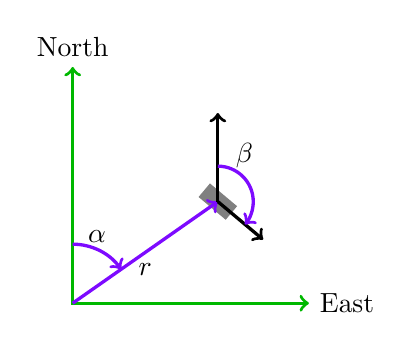
\begin{tikzpicture}[scale=1.5,line width=1.2pt]

  \definecolor{enu}{RGB}{0,184,0} % green
  \definecolor{compass}{RGB}{125,10,255} % purple
  \definecolor{base}{RGB}{128,128,128} % grey

  % Origin
  \coordinate (o) at (0,0);

  % Draw ENU axes
  \draw [enu,<->]
      (0,2) node[black] (yaxis) [above] {North} |-
      (2,0) node[black] (xaxis) [right] {East};

  % Draw a detectors
  \coordinate (d0) at (35:1.5);
  \fill[base,rotate=-40] (d0) ++(-.15,-.075) rectangle +(.3,.15);

  % Draw distance line
  \draw[compass,->] (o) -- node[black,below] {$r$} (d0);
  % Draw angle line
  \draw[compass,->] (0,.5) arc (90:35:.5);
  \draw[compass] (70:.6) node[black] {$\alpha$};

  % Draw North from detector
  \draw[->] (d0) -- +(0,.75);
  % Draw detector angle
  \draw[->] (d0) -- +(-40:.5);

  % Draw angle line
  \draw[compass,->] (d0) ++(0,.3) arc (90:-40:.3);
  \draw[compass] (d0) ++(60:.45) node[black] {$\beta$};

\end{tikzpicture}

    \caption{Relationship ENU (green) and compass (purple) coordinate system
             and how it is used to define the position of a detector.}
    \label{fig:enu_compass}
\end{figure}


\section{Celestial}

\subsection{Azimuth and Zenith}

When a station detects a shower we try to reconstruct the direction of
its origin. The direction of a shower is then given by an azimuth and
zenith coordinate. These coordinates define a point on the semi-sphere
that is the sky above the detection station. The zenith is the point
directly above the observer. The zenith angle is the angle between the
direction and the zenith point. The azimuth is the direction in the
horizontal plane, it starts at East then goes to North (ENWS).

We do not expect nor consider air showers from below the horizon, so the
zenith angles, defined in radians, are and angle in the range (0,
$\frac{\pi}{2}$). The azimuth is restricted to the range ($-\pi$, $\pi$).


\subsection{Horizontal}

This is a system used as intermediary for some coordinate conversions.
It uses azimuth and altitude to define a direction. The altitude is the
opposite of the zenith, so 0 is horizontal and $\frac{\pi}{2}$ is the
zenith. The azimuth definition also differs, it moves from North to East
(NESW).


\subsection{Equatorial (J2000)}

Vernal equinox, epoch.
Right ascension, Declination, J2000
In decimal hours.


\section{\corsika}

\cite{corsika}

\subsection{Geographic}

\corsika defines positions on the ground (or observation level) relative
to the core of the shower(??). Positive x axis points to magnetic North,
positive y axis to the West, and the z axis upwards.


\subsection{Celestial}

As origin of the shower \corsika looks from the point of view of the
shower. The $\theta$ angle is defined the same as our definition of
zenith, \SI{0}{\radian} is a shower from the zenith and
\SI{\pi / 2}{\radian} is a horizontal shower. The $\phi$ angle is
defined differently than our definition of azimuth. First it is the
angle the shower is heading towards. \SI{0}{\radian} is a shower heading
towards North, so coming form South, which we would define as
\SI{\pi / 2}{\radian}. The (positive) rotation of the angle is
in the same direction, from North to West. So the conversion is:.


\bibliography{References}

\begin{thebibliography}{9}

\bibitem{wikigeodetic}
Geodetic system. In Wikipedia. Retrieved August 10, 2004,
from \url{http://en.wikipedia.org/wiki/Geodetic_system}

\bibitem{corsika}
Corsika manual Chapter 6 Coordinate System.

\end{thebibliography}
